\newcommand{\sdssbandtable}{\begin{tabular}{|c|D{.}{.}{3.2}|D{.}{.}{3.2}|D{.}{.}{3.2}|D{.}{.}{3.2}|D{.}{.}{3.2}|}
\hline
\multicolumn{1}{|c|}{\textbf{CPU time}} &\multicolumn{5}{c|}{\textbf{Percentage of images recognized}} \\
\cline{2-6}
\multicolumn{1}{|c|}{(per image)} & \multicolumn{1}{c|}{$u$} & \multicolumn{1}{c|}{$g$} & \multicolumn{1}{c|}{$r$} & \multicolumn{1}{c|}{$i$} & \multicolumn{1}{c|}{$z$} \\
\hline
\makebox[\pointonesec][r]{$0.1$ s} & 87.80  & 93.88  & 94.87  & 93.59  & 94.36 \\
\makebox[\pointonesec][r]{$1$ s} & 98.58  & 99.73  & 99.78  & 99.73  & 99.75 \\
\makebox[\pointonesec][r]{$10$ s} & 99.82  & 99.96  & 99.97  & 99.96  & 99.96 \\
\makebox[\pointonesec][r]{$60$ s} & 99.84  & 99.96  & 99.97  & 99.96  & 99.96 \\
\hline
\end{tabular}
}
\newcommand{\sdssbandsobjsfig}{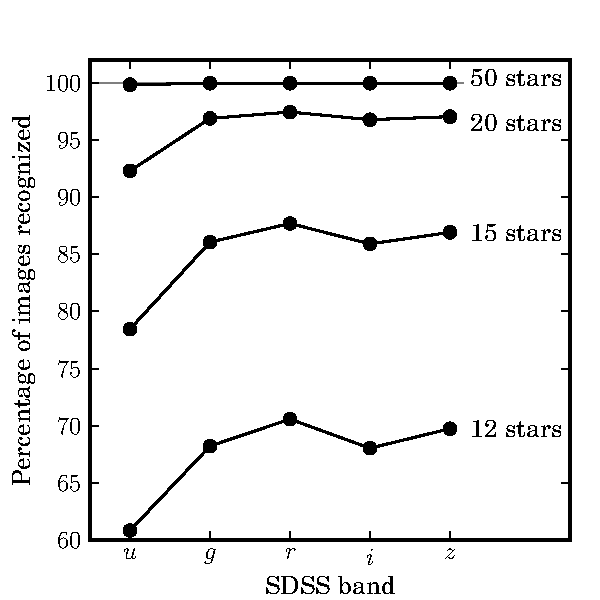
\includegraphics[width=1.000000\figunit]{sdss-bands-objs}}
\newcommand{\sdssbandstimefig}{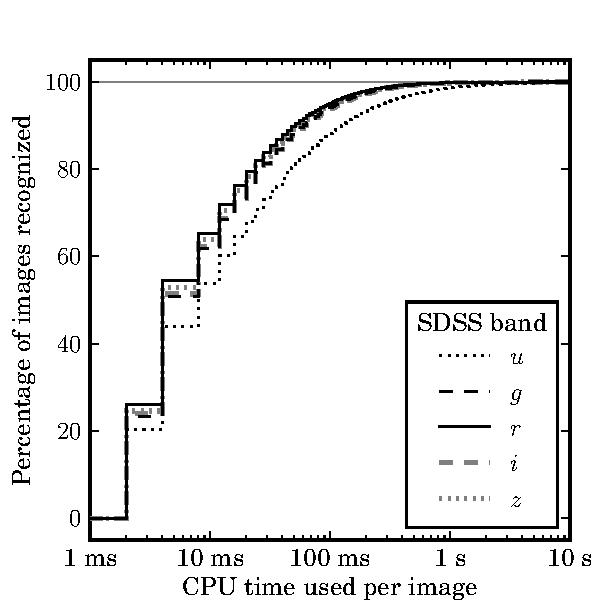
\includegraphics[width=1.000000\figunit]{sdss-bands-time}}
